\PassOptionsToPackage{unicode=true}{hyperref} % options for packages loaded elsewhere
\PassOptionsToPackage{hyphens}{url}
%
\documentclass[]{article}
\usepackage{lmodern}
\usepackage{amssymb,amsmath}
\usepackage{ifxetex,ifluatex}
\usepackage{fixltx2e} % provides \textsubscript
\ifnum 0\ifxetex 1\fi\ifluatex 1\fi=0 % if pdftex
  \usepackage[T1]{fontenc}
  \usepackage[utf8]{inputenc}
  \usepackage{textcomp} % provides euro and other symbols
\else % if luatex or xelatex
  \usepackage{unicode-math}
  \defaultfontfeatures{Ligatures=TeX,Scale=MatchLowercase}
\fi
% use upquote if available, for straight quotes in verbatim environments
\IfFileExists{upquote.sty}{\usepackage{upquote}}{}
% use microtype if available
\IfFileExists{microtype.sty}{%
\usepackage[]{microtype}
\UseMicrotypeSet[protrusion]{basicmath} % disable protrusion for tt fonts
}{}
\IfFileExists{parskip.sty}{%
\usepackage{parskip}
}{% else
\setlength{\parindent}{0pt}
\setlength{\parskip}{6pt plus 2pt minus 1pt}
}
\usepackage{hyperref}
\hypersetup{
            pdftitle={Me and GMM covariance},
            pdfauthor={Elena Grassi},
            pdfborder={0 0 0},
            breaklinks=true}
\urlstyle{same}  % don't use monospace font for urls
\usepackage[margin=1in]{geometry}
\usepackage{color}
\usepackage{fancyvrb}
\newcommand{\VerbBar}{|}
\newcommand{\VERB}{\Verb[commandchars=\\\{\}]}
\DefineVerbatimEnvironment{Highlighting}{Verbatim}{commandchars=\\\{\}}
% Add ',fontsize=\small' for more characters per line
\usepackage{framed}
\definecolor{shadecolor}{RGB}{248,248,248}
\newenvironment{Shaded}{\begin{snugshade}}{\end{snugshade}}
\newcommand{\AlertTok}[1]{\textcolor[rgb]{0.94,0.16,0.16}{#1}}
\newcommand{\AnnotationTok}[1]{\textcolor[rgb]{0.56,0.35,0.01}{\textbf{\textit{#1}}}}
\newcommand{\AttributeTok}[1]{\textcolor[rgb]{0.77,0.63,0.00}{#1}}
\newcommand{\BaseNTok}[1]{\textcolor[rgb]{0.00,0.00,0.81}{#1}}
\newcommand{\BuiltInTok}[1]{#1}
\newcommand{\CharTok}[1]{\textcolor[rgb]{0.31,0.60,0.02}{#1}}
\newcommand{\CommentTok}[1]{\textcolor[rgb]{0.56,0.35,0.01}{\textit{#1}}}
\newcommand{\CommentVarTok}[1]{\textcolor[rgb]{0.56,0.35,0.01}{\textbf{\textit{#1}}}}
\newcommand{\ConstantTok}[1]{\textcolor[rgb]{0.00,0.00,0.00}{#1}}
\newcommand{\ControlFlowTok}[1]{\textcolor[rgb]{0.13,0.29,0.53}{\textbf{#1}}}
\newcommand{\DataTypeTok}[1]{\textcolor[rgb]{0.13,0.29,0.53}{#1}}
\newcommand{\DecValTok}[1]{\textcolor[rgb]{0.00,0.00,0.81}{#1}}
\newcommand{\DocumentationTok}[1]{\textcolor[rgb]{0.56,0.35,0.01}{\textbf{\textit{#1}}}}
\newcommand{\ErrorTok}[1]{\textcolor[rgb]{0.64,0.00,0.00}{\textbf{#1}}}
\newcommand{\ExtensionTok}[1]{#1}
\newcommand{\FloatTok}[1]{\textcolor[rgb]{0.00,0.00,0.81}{#1}}
\newcommand{\FunctionTok}[1]{\textcolor[rgb]{0.00,0.00,0.00}{#1}}
\newcommand{\ImportTok}[1]{#1}
\newcommand{\InformationTok}[1]{\textcolor[rgb]{0.56,0.35,0.01}{\textbf{\textit{#1}}}}
\newcommand{\KeywordTok}[1]{\textcolor[rgb]{0.13,0.29,0.53}{\textbf{#1}}}
\newcommand{\NormalTok}[1]{#1}
\newcommand{\OperatorTok}[1]{\textcolor[rgb]{0.81,0.36,0.00}{\textbf{#1}}}
\newcommand{\OtherTok}[1]{\textcolor[rgb]{0.56,0.35,0.01}{#1}}
\newcommand{\PreprocessorTok}[1]{\textcolor[rgb]{0.56,0.35,0.01}{\textit{#1}}}
\newcommand{\RegionMarkerTok}[1]{#1}
\newcommand{\SpecialCharTok}[1]{\textcolor[rgb]{0.00,0.00,0.00}{#1}}
\newcommand{\SpecialStringTok}[1]{\textcolor[rgb]{0.31,0.60,0.02}{#1}}
\newcommand{\StringTok}[1]{\textcolor[rgb]{0.31,0.60,0.02}{#1}}
\newcommand{\VariableTok}[1]{\textcolor[rgb]{0.00,0.00,0.00}{#1}}
\newcommand{\VerbatimStringTok}[1]{\textcolor[rgb]{0.31,0.60,0.02}{#1}}
\newcommand{\WarningTok}[1]{\textcolor[rgb]{0.56,0.35,0.01}{\textbf{\textit{#1}}}}
\usepackage{graphicx,grffile}
\makeatletter
\def\maxwidth{\ifdim\Gin@nat@width>\linewidth\linewidth\else\Gin@nat@width\fi}
\def\maxheight{\ifdim\Gin@nat@height>\textheight\textheight\else\Gin@nat@height\fi}
\makeatother
% Scale images if necessary, so that they will not overflow the page
% margins by default, and it is still possible to overwrite the defaults
% using explicit options in \includegraphics[width, height, ...]{}
\setkeys{Gin}{width=\maxwidth,height=\maxheight,keepaspectratio}
\setlength{\emergencystretch}{3em}  % prevent overfull lines
\providecommand{\tightlist}{%
  \setlength{\itemsep}{0pt}\setlength{\parskip}{0pt}}
\setcounter{secnumdepth}{0}
% Redefines (sub)paragraphs to behave more like sections
\ifx\paragraph\undefined\else
\let\oldparagraph\paragraph
\renewcommand{\paragraph}[1]{\oldparagraph{#1}\mbox{}}
\fi
\ifx\subparagraph\undefined\else
\let\oldsubparagraph\subparagraph
\renewcommand{\subparagraph}[1]{\oldsubparagraph{#1}\mbox{}}
\fi

% set default figure placement to htbp
\makeatletter
\def\fps@figure{htbp}
\makeatother


\title{Me and GMM covariance}
\author{Elena Grassi}
\date{2/2/2023}

\begin{document}
\maketitle

\hypertarget{easy-example-in-2d-where-inside-groups-elements-are-not-correlated}{%
\subsection{Easy example in 2D where inside groups elements are not
correlated}\label{easy-example-in-2d-where-inside-groups-elements-are-not-correlated}}

\begin{Shaded}
\begin{Highlighting}[]
\NormalTok{SMALLER=}\DecValTok{300}
\NormalTok{LARGER=}\DecValTok{700}

\NormalTok{npG1 <-}\StringTok{ }\KeywordTok{rnorm}\NormalTok{(LARGER, }\DataTypeTok{mean=}\DecValTok{2}\NormalTok{, }\DataTypeTok{sd=}\DecValTok{1}\NormalTok{)}
\NormalTok{npG2 <-}\StringTok{ }\KeywordTok{rnorm}\NormalTok{(LARGER, }\DataTypeTok{mean=}\DecValTok{4}\NormalTok{, }\DataTypeTok{sd=}\FloatTok{1.5}\NormalTok{)}

\NormalTok{pG1 <-}\StringTok{ }\KeywordTok{rnorm}\NormalTok{(SMALLER, }\DataTypeTok{mean=}\DecValTok{4}\NormalTok{, }\DataTypeTok{sd=}\FloatTok{1.2}\NormalTok{)}
\NormalTok{pG2 <-}\StringTok{ }\KeywordTok{rnorm}\NormalTok{(SMALLER, }\DataTypeTok{mean=}\DecValTok{10}\NormalTok{, }\DataTypeTok{sd=}\FloatTok{1.8}\NormalTok{)}

\NormalTok{data <-}\StringTok{ }\KeywordTok{data.frame}\NormalTok{(}\DataTypeTok{G1=}\KeywordTok{c}\NormalTok{(npG1, pG1), }\DataTypeTok{G2=}\KeywordTok{c}\NormalTok{(npG2, pG2))}

\NormalTok{pan_real <-}\StringTok{ }\KeywordTok{c}\NormalTok{(}\KeywordTok{rep}\NormalTok{(}\OtherTok{FALSE}\NormalTok{, LARGER), }\KeywordTok{rep}\NormalTok{(}\OtherTok{TRUE}\NormalTok{, SMALLER))}
\KeywordTok{ggplot}\NormalTok{(data, }\KeywordTok{aes}\NormalTok{(}\DataTypeTok{x=}\NormalTok{G1, }\DataTypeTok{y=}\NormalTok{G2))}\OperatorTok{+}\KeywordTok{stat_density_2d}\NormalTok{(}\KeywordTok{aes}\NormalTok{(}\DataTypeTok{fill =} \KeywordTok{stat}\NormalTok{(level)), }\DataTypeTok{geom =} \StringTok{"polygon"}\NormalTok{)}\OperatorTok{+}\KeywordTok{theme_bw}\NormalTok{()}
\end{Highlighting}
\end{Shaded}

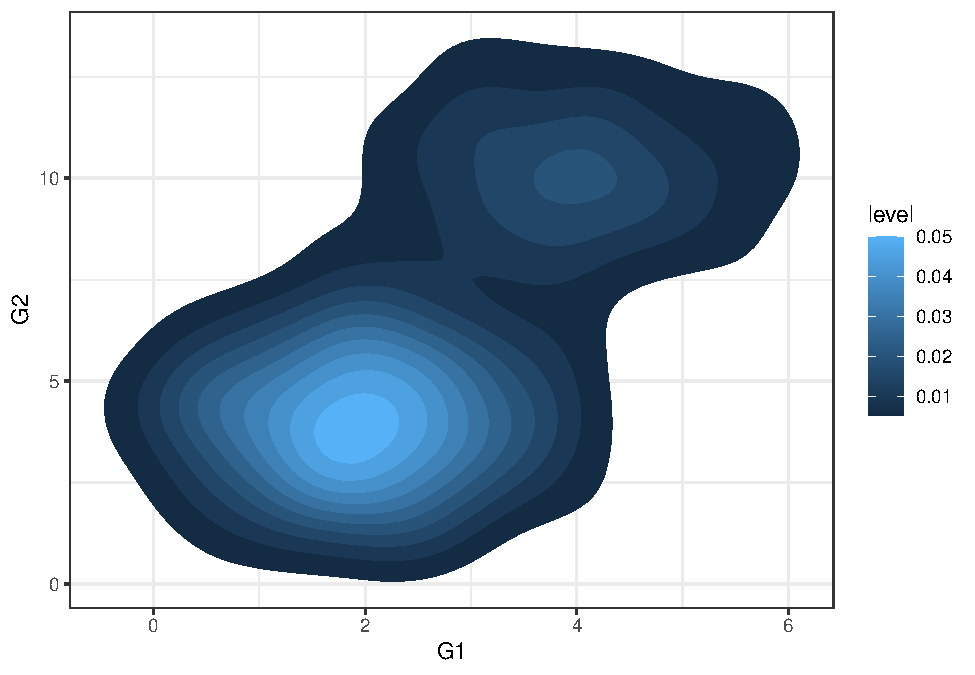
\includegraphics{covariance_gmm_files/figure-latex/data_ex_1-1.pdf}

Let's fit it with the right thing, that here is diagonal, meaning the
ellipses are inline with the x/y axes due to independence of G1 and G2
inside the two groups. Let's go with VVI! Then we'll compute the correct
answers for this model, and then try out a ``wrong'' one.

\begin{Shaded}
\begin{Highlighting}[]
\NormalTok{GMM <-}\StringTok{ }\KeywordTok{densityMclust}\NormalTok{(}\DataTypeTok{data=}\NormalTok{data, }\DataTypeTok{G=}\DecValTok{2}\NormalTok{, }\DataTypeTok{modelNames=}\StringTok{'VVI'}\NormalTok{)}
\end{Highlighting}
\end{Shaded}

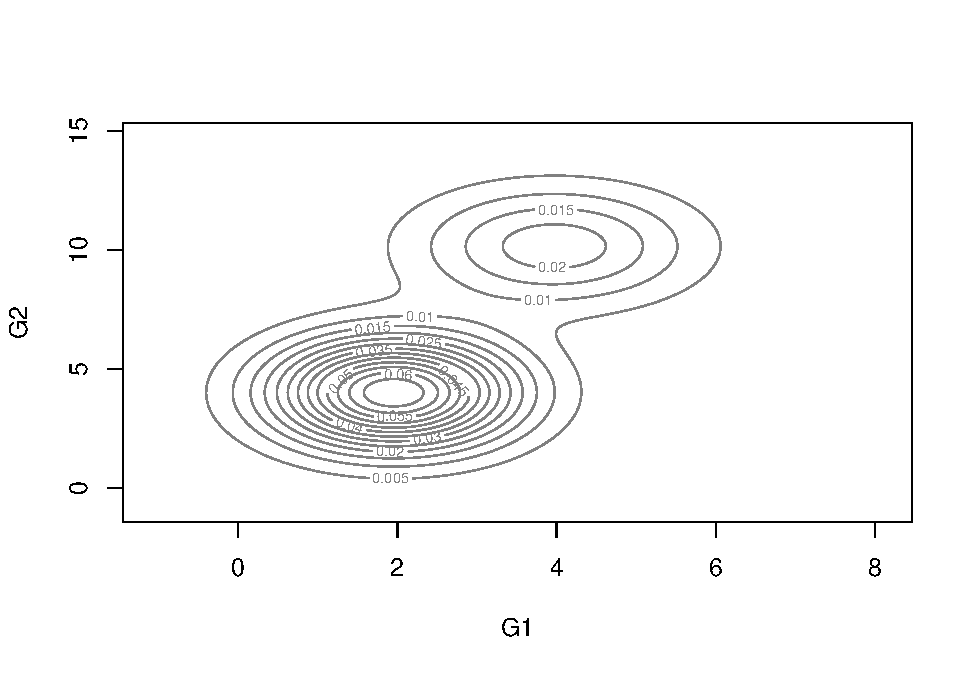
\includegraphics{covariance_gmm_files/figure-latex/fitdiag_ex1-1.pdf}

\begin{Shaded}
\begin{Highlighting}[]
\NormalTok{call_paneth <-}\StringTok{ }\ControlFlowTok{function}\NormalTok{(GMMo, }\DataTypeTok{thr=}\FloatTok{0.99}\NormalTok{) \{}
\NormalTok{  posteriors <-}\StringTok{ }\NormalTok{GMMo}\OperatorTok{$}\NormalTok{z }\CommentTok{# furtooo di codice}
\NormalTok{  mu <-}\StringTok{ }\KeywordTok{data.frame}\NormalTok{(GMMo}\OperatorTok{$}\NormalTok{parameters}\OperatorTok{$}\NormalTok{mean)}
\NormalTok{  meta_mu <-}\StringTok{ }\KeywordTok{apply}\NormalTok{(mu, }\DecValTok{2}\NormalTok{, }\ControlFlowTok{function}\NormalTok{(x) \{}\KeywordTok{exp}\NormalTok{(}\KeywordTok{mean}\NormalTok{(}\KeywordTok{log}\NormalTok{(x)))\})}
  \ControlFlowTok{if}\NormalTok{ (meta_mu[[}\DecValTok{1}\NormalTok{]][}\DecValTok{1}\NormalTok{] }\OperatorTok{>}\StringTok{ }\NormalTok{meta_mu[[}\DecValTok{2}\NormalTok{]][}\DecValTok{1}\NormalTok{]) \{}
    \KeywordTok{colnames}\NormalTok{(posteriors)<-}\KeywordTok{list}\NormalTok{(}\StringTok{"p(paneth)"}\NormalTok{,}\StringTok{"p(non_paneth)"}\NormalTok{)}
\NormalTok{  \} }\ControlFlowTok{else}\NormalTok{ \{}
    \KeywordTok{colnames}\NormalTok{(posteriors)<-}\KeywordTok{list}\NormalTok{(}\StringTok{"p(non_paneth)"}\NormalTok{,}\StringTok{"p(paneth)"}\NormalTok{)}
\NormalTok{  \}}
\NormalTok{  posteriors[,}\StringTok{'p(paneth)'}\NormalTok{] }\OperatorTok{>}\StringTok{ }\NormalTok{thr}
\NormalTok{\}}

\NormalTok{pan <-}\StringTok{ }\KeywordTok{call_paneth}\NormalTok{(GMM)}
\KeywordTok{table}\NormalTok{(pan, pan_real)}
\end{Highlighting}
\end{Shaded}

\begin{verbatim}
##        pan_real
## pan     FALSE TRUE
##   FALSE   700   56
##   TRUE      0  244
\end{verbatim}

Uh, it seems I created a bad example, but I will finish working on it,
then we can decide if we want to refine it to me more similar to real
life. Let's see how the full model, VVV, works here.

\begin{Shaded}
\begin{Highlighting}[]
\NormalTok{GMM <-}\StringTok{ }\KeywordTok{densityMclust}\NormalTok{(}\DataTypeTok{data=}\NormalTok{data, }\DataTypeTok{G=}\DecValTok{2}\NormalTok{, }\DataTypeTok{modelNames=}\StringTok{'VVV'}\NormalTok{)}
\end{Highlighting}
\end{Shaded}

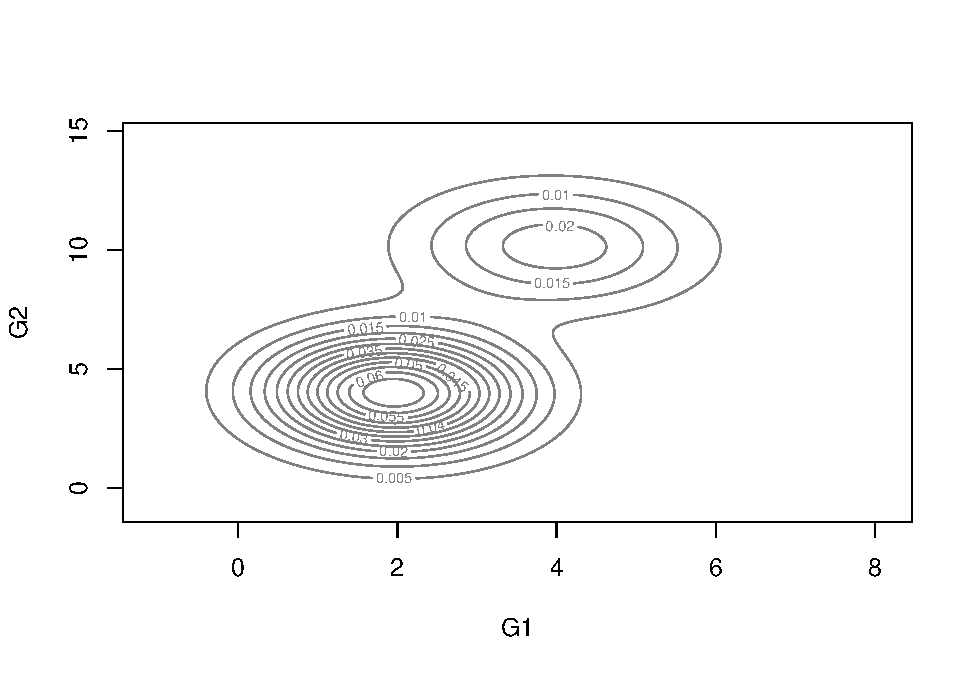
\includegraphics{covariance_gmm_files/figure-latex/fitfull_ex1-1.pdf}

\begin{Shaded}
\begin{Highlighting}[]
\NormalTok{pan <-}\StringTok{ }\KeywordTok{call_paneth}\NormalTok{(GMM)}
\KeywordTok{table}\NormalTok{(pan, pan_real)}
\end{Highlighting}
\end{Shaded}

\begin{verbatim}
##        pan_real
## pan     FALSE TRUE
##   FALSE   700   53
##   TRUE      0  247
\end{verbatim}

OK, I'm confused\ldots{}I was expecting it to be worse!

\hypertarget{example-n.2-what-if-we-have-the-dreaded-correlation-inside-groups}{%
\subsection{Example n.2: what if we have the dreaded correlation inside
groups?}\label{example-n.2-what-if-we-have-the-dreaded-correlation-inside-groups}}

Let's say they are only in the Paneth cells!

\begin{Shaded}
\begin{Highlighting}[]
\NormalTok{npG1 <-}\StringTok{ }\KeywordTok{rnorm}\NormalTok{(LARGER, }\DataTypeTok{mean=}\DecValTok{2}\NormalTok{, }\DataTypeTok{sd=}\DecValTok{1}\NormalTok{)}
\NormalTok{npG2 <-}\StringTok{ }\KeywordTok{rnorm}\NormalTok{(npG2, }\DataTypeTok{mean=}\DecValTok{4}\NormalTok{, }\DataTypeTok{sd=}\FloatTok{1.5}\NormalTok{)}

\NormalTok{pG1 <-}\StringTok{ }\KeywordTok{rnorm}\NormalTok{(SMALLER, }\DataTypeTok{mean=}\DecValTok{4}\NormalTok{, }\DataTypeTok{sd=}\FloatTok{1.2}\NormalTok{)}
\NormalTok{pG2 <-}\StringTok{ }\NormalTok{pG1}\OperatorTok{*}\FloatTok{1.5}\OperatorTok{+}\KeywordTok{jitter}\NormalTok{(pG1)}

\NormalTok{data2 <-}\StringTok{ }\KeywordTok{data.frame}\NormalTok{(}\DataTypeTok{G1=}\KeywordTok{c}\NormalTok{(npG1, pG1), }\DataTypeTok{G2=}\KeywordTok{c}\NormalTok{(npG2, pG2))}

\KeywordTok{ggplot}\NormalTok{(data2, }\KeywordTok{aes}\NormalTok{(}\DataTypeTok{x=}\NormalTok{G1, }\DataTypeTok{y=}\NormalTok{G2))}\OperatorTok{+}\KeywordTok{stat_density_2d}\NormalTok{(}\KeywordTok{aes}\NormalTok{(}\DataTypeTok{fill =} \KeywordTok{stat}\NormalTok{(level)), }\DataTypeTok{geom =} \StringTok{"polygon"}\NormalTok{)}\OperatorTok{+}\KeywordTok{theme_bw}\NormalTok{()}
\end{Highlighting}
\end{Shaded}

\includegraphics{covariance_gmm_files/figure-latex/data_ex_2-1.pdf}

\begin{Shaded}
\begin{Highlighting}[]
\NormalTok{GMM <-}\StringTok{ }\KeywordTok{densityMclust}\NormalTok{(}\DataTypeTok{data=}\NormalTok{data2, }\DataTypeTok{G=}\DecValTok{2}\NormalTok{, }\DataTypeTok{modelNames=}\StringTok{'VVI'}\NormalTok{)}
\end{Highlighting}
\end{Shaded}

\includegraphics{covariance_gmm_files/figure-latex/fitdiag_ex2-1.pdf}

\begin{Shaded}
\begin{Highlighting}[]
\NormalTok{pan <-}\StringTok{ }\KeywordTok{call_paneth}\NormalTok{(GMM)}
\KeywordTok{table}\NormalTok{(pan, pan_real)}
\end{Highlighting}
\end{Shaded}

\begin{verbatim}
##        pan_real
## pan     FALSE TRUE
##   FALSE   700  127
##   TRUE      0  173
\end{verbatim}

\begin{Shaded}
\begin{Highlighting}[]
\NormalTok{GMM <-}\StringTok{ }\KeywordTok{densityMclust}\NormalTok{(}\DataTypeTok{data=}\NormalTok{data2, }\DataTypeTok{G=}\DecValTok{2}\NormalTok{, }\DataTypeTok{modelNames=}\StringTok{'VVV'}\NormalTok{)}
\end{Highlighting}
\end{Shaded}

\includegraphics{covariance_gmm_files/figure-latex/fitfull_ex2-1.pdf}

\begin{Shaded}
\begin{Highlighting}[]
\NormalTok{pan <-}\StringTok{ }\KeywordTok{call_paneth}\NormalTok{(GMM)}
\KeywordTok{table}\NormalTok{(pan, pan_real)}
\end{Highlighting}
\end{Shaded}

\begin{verbatim}
##        pan_real
## pan     FALSE TRUE
##   FALSE   700    0
##   TRUE      0  300
\end{verbatim}

\end{document}
